% ------------------------------------------------------------------------
% file `1_E_juin-appliquer-18-exercise-body.tex'
%   in folder `xsim/'
%
%     exercise of type `appliquer' with id `18'
%
% generated by the `appliquer' environment of the
%   `xsim' package v0.20c (2021/02/03)
% from source `1_E_juin' on 2023/06/06 on line 379
% ------------------------------------------------------------------------
    Voici un repère cartésien. \\
    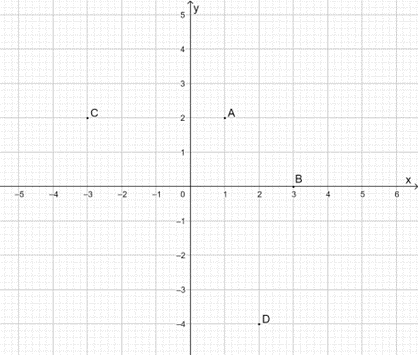
\includegraphics{img/graphe.png}
    \begin{enumerate}
        \item Écris les coordonnées des points suivants. \\
              \(A(\ldots; \ldots)\) \hfill \(B(\ldots; \ldots)\) \hfill  \(C(\ldots; \ldots)\) \hfill  \(D(\ldots; \ldots)\)
        \item Place le point \(X\) tel que \(X(-5;-2)\)
        \item Complète les phrases suivantes par \(A, B, C\) ou \(D\).
              %\begin{enumitem} \TODO: enumitem (TITI : je ne comprends pas)
        \item Mon ordonnée vaut le double de mon abscisse, je suis le point \dotfill
        \item Nous avons la même ordonnée, nous sommes les points \dotfill
              %\end{enumitem}
    \end{enumerate}
